\documentclass[11pt]{article}
\def\StudentVersion{}
\usepackage{../common}
\usepackage{pdfpages}
\usepackage{proof}


\title{Propositional Logic and Planning}
\date{}

\def\LecStr{Alexander Rush}
\def\LecNum{4}
\def\LecTitle{Lecture Notes on Propositional Logic}
\def\LecDate{}

\begin{document}
\MakeScribeTop{}
\tableofcontents

\section{Introduction}

One of the central goals of artificial intelligence is to be able to
model human reasoning. We would expect a reasoning agent to be able to
start with a set of knowledge and be able to draw conclusions about
the statements relating to this input. This task seems quite far from
our previous two units on search and constraint satisfaction, although we will see that it is closely related.

In the next few lectures  we will explicitly discuss the task of reasoning about knowledge. We
introduce a very simple form of a logic known as propositional logic,
and show how it can be used to encode sets of facts, known
as knowledge bases. We then show how to use these knowledge bases to
reason about new statements. To do this we will transform the logical
representation into a form that again allows us to use the tools and
language of search. We finish with a brief survey of the area of
\textbf{planning}, which uses a logical representation to reason about
sequences of events.

\section{A Running Example: Medical Diagnosis}

Consider the following flowchart distributed to help people with flu-like symptoms to perform self-diagnostics. 

\includepdf{flu_selfassess_flowchart}

\noindent If we treat the state of a patient and the recommended action as a set of possible worlds, this chart can be seen as a knowledge base in propositional logic which will be the main focus of this note.  

For simplicity let's cut down the number of possible symptoms to around 10.  
In English, we can roughly interpret these statements as saying:

\begin{itemize}
\item  You may have the flu only if you have a cough in addition to a fever or are sweating. 
\item  If you may have the flu and you have confusion or vomiting then call the emergency room.
\item  If you may have the flu but don't think it's an emergency, and you are over 65, then call the doctor.
\end{itemize}

It allows us to ask and answer formal questions about the structure of the world. 
For instance we might wonder:

\begin{itemize}
\item If I may have the flu does this mean that I am sweaty?
\end{itemize}

\noindent When we return to this example, we will see algorithms that allow us to
answer these types of queries.

\section{Propositional Logic}

\subsection{The Logic Framework}

In this class we'll be considering a simple variant of
\textbf{formal logic}.  In this framework we assume that there is an
underlying state of the world which is completely described by a
\textbf{model} (used here in a formal sense). For now, we will treat the model $m$ abstractly as
some member of the set of all possible worlds $\mcM$. In the next
section we will explicitly define the type of models of interest.

Logic allows us to make statements about the world, which we will call
sentences.  Under some worlds a sentence $\alpha$ may evaluate to
true, and in others it may evaluate to false.  In the first case (true), we
say that the model \textbf{satisfies} the sentence. We use the
notation $\mcM(\alpha)$ to specify all the subset of models that satisfy a given
sentence $\alpah$.

We can also consider the relationship between two logical sentences
$\alpha$ and $\beta$.  If the statement $\alpha$ implies that $\beta$
is true, we say $\alpha$ \textbf{entails} $\beta$ and write this as
$\alpha \models \beta$.The entailment relationship can be defined set-theoretically using
models.  Formally: \[\alpha \models \beta \mathrm{\ iff\ } \mcM(\alpha)
\subset \mcM(\beta),\] \noindent That is $\alpha$ entails $\beta$ is all models satisfied by $\alpha$ are
also satisfied by $\beta$.
   
In practice we will very rarely be able to enumerate all the possible worlds in order to 
check entailment relations. However this provides an important vocabulary for thinking about the 
underlying assumptions of formal logic.


\subsection{Syntax and Semantics of Propositional Logic}

Now we look at specific variant of logic known as propositional
logic. In propositional logic, we define a model as a mapping from
atomic variables to true or false. That is we assume world consists of
a set of proposition variables, and a model simply specifies
whether each specific proposition is true or false in the current world,
i.e. $m : \mcP \mapsto \{ \top, \bot\}$.

\subsection{Syntax and Semantics}

Next we define a language for constructing sentences $\alpha$ about our propositional world. Unlike natural language, the sentence will come from a language with  formally defined syntax and semantics. 
The following chart describes each of the symbols in the logic and their informal meaning.

 \air
\begin{center}
\begin{tabularx}{\linewidth}{lcX}
  \toprule

  Name & Syntax & Description \\
  \midrule \\
  literal & $P, Q$ & Reference to underlying propositions in $\mcP$ \\ 
  true &  $\top$ & Symbol for true \\ 
  false &  $\bot$ & Symbol for false \\ 
  not & $\lnot$ & $\lnot P$ is true iff $P$ is false in $m$ \\\\
  conjunction/and & $\land$ & $P \land Q$ is true iff $P$ and $Q$ is true in $m$ \\\\
  disjunction/or & $\lor$ & $P \lor Q$ is true iff $P$ or $Q$ is true in $m$ \\\\
  conditional & $\Rightarrow$& \censor{$P \Rightarrow Q$ is true unless $P$ is true and $Q$ is false in $m$} \\\\ 
  biconditional & $\Leftrightarrow$&\censor{  $P \Leftrightarrow Q$ is true iff $P$ and $Q$ are both true or both false in $m$} \\\\
 \bottomrule
\end{tabularx}
\end{center}
\air 

\noindent AIMA also gives the full specification for the grammar, order of operations, and truth table of these symbols. It generally 
follows the standard mathematical standards for these symbols. For instance here is the definition of conditional:


\air 
\begin{center}
  \begin{tabular}{lllc}
    \toprule
    P & Q && P $\Rightarrow$ Q  \\
    \midrule
    $\bot$ & $\bot$ && \censor{$\top$} \\
    $\bot$ & $\top$ && \censor{$\top$} \\
    $\top$ & $\bot$ && \censor{$\bot$} \\
    $\top$ & $\top$ && \censor{$\top$} \\
    \bottomrule
  \end{tabular}
\end{center}
\air

\subsection{Knowledge Base}

Using a logical formalism we can define a knowledge base (KB) as a collection of 
conjoined ($\land$) sentences from the formalism. Implicitly our knowledge base $KB$
defines the set of worlds $\mcM(KB)$ of interest. 

Once we have a knowledge base, we can issue \textbf{queries} $\alpha$ consisting of logical 
statements about the knowledge base. In particular we will be interested in whether 
the knowledge base entails the question, i.e. $KB \models \alpha$. 

The simplest way to do this would be to use \textbf{model checking}. Here we utilize the theory of entailment and check whether $\mcM(KB) \subset \mcM(\alpha)$. We could do this be constructing the two sets of models and confirming a subset relation, or by finding a contradiction.


\subsection{Example: Medical Diagnostics}

As a running example, we will consider the following flowchart distributed to help people with flu-like symptoms to perform informal self-diagnostics. 

% Consider the following flowchart distributed to help people with flu-like symptoms to perform self-diagnostics. 

% \includepdf{flu_selfassess_flowchart}

Now let us return to our diagnostics example. Recall that the diagram tells us the following relationship:

\begin{itemize}
\item  You may have the flu only if you have a cough in addition to a fever or are sweating. 
\item  If you may have the flu and you have confusion or vomiting then call the emergency room.
\item  If you may have the flu but don't think it's an emergency, and you are over 65, then call the doctor.
\end{itemize}

\noindent As noted above: If we treat the state of a patient and the recommended action as a set of possible worlds, this chart can be seen as a knowledge base in propositional logic.  Here's what it looks like:

\begin{eqnarray*}
 (((\msc{Fever} \lor \msc{Sweaty}) \land \msc{Cough})) &\Leftrightarrow& \msc{MayHaveFlu}) \land \\
 ((\msc{MayHaveFlu} \land (\msc{Confusion} \lor \msc{Vomiting}) &\Rightarrow& \msc{Emergency}) \land \\
 ((\msc{MayHaveFlu} \land \lnot \msc{Emergency} \land \msc{Over65}) &\Rightarrow& \msc{CallDoctor}) \\
\end{eqnarray*}

The knowledge base contains 9 propositions:

\air
\begin{center}
  \begin{tabular}{lcccc}
    \toprule
    Propositions &  $\mcM(KB)_1$ & $\mcM(KB)_2$ &  $\mcM(KB)_3$ & \ldots  \\
    \midrule
    \textsc{Cough}    & $\bot$ & $\top$ &  $\top$ & \\ 
    \textsc{Sweaty}   & $\bot$ & $\top$ & $\bot$ &\\ 
    \textsc{Fever}    & $\bot$ & $\bot$& $\top$ &\\ 
    \textsc{Confusion}& $\bot$ & $\bot$& $\bot$ &\\ 
    \textsc{Vomiting} & $\bot$ & $\bot$&$\bot$ &\\ 
    \textsc{Over65}   & $\bot$ & $\bot$&$\bot$ & \\ 
    \midrule
    \textsc{MayHaveFlu} & $\bot$ & $\top$&$\top$ &\\ 
    \textsc{Emergency} & $\bot$  & $\bot$&$\bot$ &\\ 
    \textsc{CallDoctor} & $\bot$ & $\bot$  &$\bot$ &\\ 
    \bottomrule
  \end{tabular}
\end{center}



\begin{exercise}
  How many possible worlds exist, what is the size of $|\mcM|$? 
\end{exercise}

\censor{This means there are a total of $|\mcM| = 2^11$.}



\noindent We could in theory enumerate all models that satisfy this $KB$, however we will see that there are easier ways to do reasoning. 

As an example consider a query $\alpha$ we might issue to this knowledge base, 

\begin{itemize}
\item If I may have the flu does this imply that I am sweaty?
\end{itemize}


 % We could in theory enumerate all models that satisfy this $KB$, however we will see that there are easier ways to do reasoning. 

As an example, consider a query  $\alpha$ we might issue to this knowledge base: ``if I may have the flu does this imply that I am sweaty''?  


Model checking method would enumerate all
models that are consistent with the KB and the query. If $M(\alpha)
\subset \mcM(KB)$ then it is entailed. Conversely, if we can find a model that is in $\mcM(KB)$ but violates
the sentence they we can conclude the opposite. 


\begin{exercise}
  Does $KB \models \alpha$?
\end{exercise}

\censor{In this case
$\mcM(KB)_3$ has $\msc{MayHaveFlu}=\top$ but has $\msc{Sweaty} = \bot$
which is a contradiction. So this query is not entailed.}

\section{Inference}

As an alternative to model-based reasoning we can instead perform
reasoning based on \textbf{inferences}.  Starting from a knowledge
base $KB$ we will attempt to transform the logical representation to
find our goal sentence $\alpha$. We can do this by applying a set of 
classical inference \textbf{rules}.


An inference rule takes a set of premises and returns a new sentence as a conclusion:

\[ \infer{\mathrm{conclusion}}{\mathrm{premise1} & \mathrm{premise2}}\]  

\noindent We can extend the set of knowledge by applying inference rules to the current data. For instance 
the simplest inference \textbf{modus ponens} or implication elimination adds the conclusion of a conditional:

\[
  \infer{\beta} {\alpha \Rightarrow \beta & \alpha}
\]

\noindent Another is simply eliminating a conjuntion:

\[
  \infer{\alpha} {\alpha \land \beta}
\]

\noindent  We can also express DeMorgan's laws as inferences:

\[
  \infer{\lnot \alpha \lor \lnot \beta} {\lnot (\alpha \land \beta)}
\]


\subsection{Search and Inference}

Using these rules we can define a search problem. This brings us back to our trusty search specification.


 \air
\begin{center}
\begin{tabularx}{\linewidth}{llX}
  \toprule
  Name  & Type & Description \\
  \midrule
\\

State &  & \censor{A conjunction of sentences} \\\\
Initial state & &  \censor{The initial knowledge base.} \\\\
Actions && \censor{All possible applications of inference rules to the knowledge base.}\\\\
Result && \censor{The transformed knowledge base.} \\\\
 Goal && \censor{Is the query in the knowledge base?} \\\\
 \bottomrule
\end{tabularx}
\end{center}

There are two desirable properties of inference rules. 


  \begin{defn}
    A rule is \textbf{sound} if it is truth preserving, i.e. it does not change the set of 
    models.
  \end{defn}

  \begin{defn}
    A set of rules is \textbf{complete} if they are guaranteed to find a solution, when used with a complete search algorithm
  \end{defn}
  

AIMA gives a set of sound rules for propositional logic and an
informal assertion that they are complete. However there is much
simpler cleaner inference strategy for dealing with propositional
logic.


\section{Resolution}

An even better method than searching with inference rules to is to use resolution. Instead of trying to produce the query, resolution
instead aims to find a \textbf{proof by contradiction}.  It first
assumes the negation of the query, and then tries to find a 
contradiction. Formally, define any sentence $\alpha$ as \textbf{satisfiable} if
there exists a model for which it is true, i.e. $\mcM(\alpha)$ is not
empty. We can then find entailment using the rule:

\[\alpha \models \beta\mathrm{\ iff\ } (\alpha \land \lnot \beta) \mathrm{\ is \ unsatisfiable}\] 

\noindent For \textbf{resolution}, for a query $\alpha$ and knowledge base KB, we first construct $KB \land \lnot \alpha$ and then search for a proof of unsatisfiability. 

% Instead of reasoning over the sets of models which can be very large, we instead consider trying to find a contradiction. This is known as proof by \textbf{resolution}. 


\subsection{Resolution for Propositional Logic}

Our aim for resolution will be to produce a contradiction of the form $p \land \lnot p$, where $p$ is a literal. We will do this by adding more sentences to the KB until we discover a contradiction or run out of inference rules to apply.

Consider a sentence in the KB consisting of a disjunction of possibly negated literals $l_1 \lor \ldots \lor l_k$. We call this a \textbf{clause}. If we also know from the KB that any of the literals are false, i.e. $\lnot l_i$ , we can remove it from the list, producing a smaller disjunctive clause. This is called a \textbf{unit resolution}:

\[
  \infer{l_1 \lor \ldots \lor
    l_{i-1} \lor l_{i+1} \lor \ldots \lor l_k }{l_1 \lor \ldots
    \lor l_k &  \lnot l_i}.
\]


\noindent However we don't need to just do unit resolutions, if there is a another clause $m_1 \lor \ldots \lor m_n$ that contains the negation of any literal in $l$ then we can soundly resolve the two clauses. This is called \textbf{general resolution}:

\air

\censorm{
\[
  \infer[\mathrm{\ where\ } l_i = \lnot m_j]{l_1 \lor \ldots \lor
    l_{i-1} \lor l_{i+1} \lor \ldots \lor l_k \lor m_1 \lor \ldots
    \lor m_{j-1} \lor m_{j+1}\lor \ldots \lor m_n }{l_1 \lor \ldots
    \lor l_k & m_1 \lor \ldots \lor m_n}
\]
}
\air 

The key idea of propositional resolution is that if the KB only consists of clauses, then general resolution is the only inference rule needed to produce a complete inference algorithm.

% It turns that this is the only inference rule actually necessary. It turns out with just resolution we have the two properties we need:

\begin{itemize}
\item Soundness: The resolution rule is truth preserving
  
\item Completeness: It is always able to find a proof.
\end{itemize}

\noindent But what about all the other elements besides disjunction ($\lor$) and literal negation ($\lnot$)? Well it turns out we can apply a transformation that removes these elements from the problem entirely. 

\subsection{Conjunctive normal form}

Conjunctive normal formal (CNF) is a general representation for propositional logic, that consists only of conjoined clauses with propositions or negative propositions. While much more difficult to read than general propositional logic, it can represent all possible propositional sentences.  To convert a sentence in propositional logic to CNF we apply the following 4 transfomations.

\begin{enumerate}
\item Biconditional Elimination: Replace $\alpha \Leftrightarrow \beta$ with $(\alpha \Rightarrow \beta) \land(\beta \Rightarrow \alpha)$  
\item Conditional Elimination: Replace $\alpha \Rightarrow \beta$ with $\lnot \alpha \lor \beta$.
\item Move $\lnot$ inward. Demorgan's rules 

\[ \lnot (\alpha \land \beta) \triangleq (\lnot \alpha \lor \lnot \beta) \] 
\[ \lnot (\alpha \lor \beta) \triangleq (\lnot \alpha \land \lnot \beta) \] 
\item Distribute $\lor$ over $\land$.   

\[ \alpha \lor (\beta \land \gamma) \triangleq (\alpha \lor \beta)\land (\alpha \lor \gamma)\] 
\end{enumerate}

The final form of the KB will now be a conjunction of disjunctive clauses. That is a conjunction of phrases each containing only $\lor$ and $\lnot$ applied to atomic propositions.    


\paragraph{Example}

Let's convert the medical KB into CNF:

\begin{itemize}
\item Original
\begin{eqnarray*}
 (((\msc{Fever} \lor \msc{Sweaty}) \land \msc{Cough}) &\Leftrightarrow& \msc{MayHaveFlu}) \land \\
 ((\msc{MayHaveFlu} \land (\msc{Confusion} \lor \msc{Vomiting}) &\Rightarrow& \msc{Emergency}) \land\\
 ((\msc{MayHaveFlu} \land \lnot \msc{Emergency} \land \msc{Over65} &\Rightarrow& \msc{CallDoctor}) \\
\end{eqnarray*}

\item Step 1
Biconditional
\begin{eqnarray*}
 \msc{MayHaveFlu}  &\Rightarrow& ((\msc{Fever} \lor \msc{Sweaty}) \land \msc{Cough})  \land \\
 ((\msc{Fever} \lor \msc{Sweaty}) \land \msc{Cough}) &\Rightarrow& \msc{MayHaveFlu} \land \\
 (\msc{MayHaveFlu} \land (\msc{Confusion} \lor \msc{Vomiting}) &\Rightarrow& \msc{Emergency}\land \\
 (\msc{MayHaveFlu} \land \lnot \msc{Emergency} \land \msc{Over65}) &\Rightarrow& \msc{CallDoctor} \\
\end{eqnarray*}

\item Step 2
Conditional

\vspace{2cm}

\censorm{
\begin{eqnarray*}
 (\lnot \msc{MayHaveFlu}  &\lor& ((\msc{Fever} \lor \msc{Sweaty}) \land \msc{Cough}))  \land \\
 (\lnot ((\msc{Fever} \lor \msc{Sweaty}) \land \msc{Cough}) &\lor& \msc{MayHaveFlu}) \land \\
 (\lnot (\msc{MayHaveFlu} \land (\msc{Confusion} \lor \msc{Vomiting}) &\lor& \msc{Emergency})\land \\
 (\lnot (\msc{MayHaveFlu} \land \lnot \msc{Emergency} \land \msc{Over65}) &\lor& \msc{CallDoctor})\\
\end{eqnarray*}
}

\item Step 3
De Morgan's Laws
\begin{eqnarray*}
 (\lnot \msc{MayHaveFlu}  &\lor& ((\msc{Fever} \lor \msc{Sweaty}) \land \msc{Cough}))  \land \\
 ( (\lnot \msc{Fever} \land  \lnot \msc{Sweaty}) \lor \lnot \msc{Cough}) &\lor& \msc{MayHaveFlu}) \land \\
 ( ( \lnot \msc{MayHaveFlu} \lor (\lnot \msc{Confusion} \land \lnot \msc{Vomiting}) &\lor& \msc{Emergency})\land \\
 ((\lnot \msc{MayHaveFlu} \lor  \msc{Emergency} \lor \lnot \msc{Over65} &\lor& \msc{CallDoctor})\\
\end{eqnarray*}

\item Step 4 Redistribute
\begin{eqnarray*}
 ( \lnot \msc{MayHaveFlu} \lor \msc{Fever} \lor \msc{Sweaty}) \land \\
 (\lnot \msc{MayHaveFlu} \lor \msc{Cough})  \land \\
(\lnot \msc{Fever} \lor \msc{Cough} \lor \msc{MayHaveFlu}) \land \\ 
(\lnot \msc{Sweaty} \lor \msc{Cough} \lor \msc{MayHaveFlu}) \land \\ 
(\lnot \msc{Confusion} \lor \lnot \msc{MayHaveFlu} \lor \msc{Emergency}) \land \\
(\lnot \msc{Vomiting} \lor \lnot \msc{MayHaveFlu} \lor \msc{Emergency}) \land \\
  (\lnot \msc{MayHaveFlu} \lor  \msc{Emergency} \lor \lnot \msc{Over65} \lor \msc{CallDoctor})\\
\end{eqnarray*}
\end{itemize}


\noindent One step  of general resolution then yields:
\air

\[
  \infer{\censorm{\msc{Fever} \lor \msc{Sweaty}\lor \lnot \msc{Sweaty} \lor
    \msc{Cough} \lor \msc{MayHaveFlu}}}{ \lnot \msc{MayHaveFlu} \lor
    \msc{Fever} \lor \msc{Sweaty} & (\lnot \msc{Sweaty} \lor
    \msc{Cough} \lor \msc{MayHaveFlu}) }
\]
% Factoring 

% \infer{\msc{Fever}  \lor \msc{Cough} \lor \msc{MayHaveFlu}}{\msc{Fever} \lor \msc{Sweaty}\lor \lnot \msc{Sweaty} \lor \msc{Cough} \lor \msc{MayHaveFlu}}

\subsection{Resolution Algorithm}

This brings us to the full resolution algorithm for inference. 

\begin{itemize}
\item Create a new KB by adding $\lnot \alpha$, i.e. $KB \land \lnot \alpha$
\item Convert to CNF.
\item Repeatedly apply resolution.
  \begin{itemize}
  \item If there are no new clauses to resolve, the 
    KB does not entail $\alpha$.
  \item If there an empty clause is produce, we have a contradiction and KB does entail $\alpha$.
  \end{itemize}

\end{itemize}

We can show that given enough time this algorithm will either find a contradiction or find no new clauses to resolve. This gives a simple complete algorithm propositional logic. 

% So while this method is sound and complete, general CNF satisfiability is an NP-complete problem, so we cannot guarantee it will run in polynomial-time.

\textbf{However}, there is a big \textit{but} here. We have not discussed at all the complexity of this approach. This problem of determining whether a propositional statement is satisfiable is known as \textsc{Sat}. If you took CS-121 you know that a variety of this problem \textsc{3-Sat} is perhaps the most famous problem in computer science. This is one of Karp's original 21 problems, and one of the first problems to be proven NP-Complete. Therefore for general logic we can't hope to find efficient solutions. That being said there are many cases where variants of resolution and goal directed search are able to find solutions to real-world versions. 


\section{Planning}

So far we have discussed logic in the context of inference in a static world. In practice though the underlying model may be in constant flux. In planning we explicitly incorporate \textbf{actions} that change the underlying model. In many ways this is similar to the actions that occur in search. However, planning will utilize propositional logic to explictly declare exactly which actions are applicable in each state and how they update the state of the world. 

The upside of this extra information is that it will allow us to use general purpose planners to perform search. These planners can take advantage of the logical representation to generate effective heuristics for the planning search problem without requiring domain knowledge.

\subsection{Closed-World Assumption}

Before discussing planning, we need to make one change to our current
assumptions about the semantics of propositional logic, known as the
closed-world assumption. So far, we have been assuming that all propositions
in the world are explicitly included in the knowledge base. In the
closed-world assumption we allow there to be arbitrary additional
propositions, but that they are assumed to be false in all models . 

For instance in the medical diagnosis example, we might pose a 
closed world query of the form: 
 \[\msc{IsDoctor} \lor \msc{Coughing} \] 

Which would not be implied since $\msc{IsDoctor}$ is not in the knowledge-base 
and is assumed to be false and $\msc{Coughing}$ may or may not be true.

We can take this a step further and make \textbf{lifted} literals for an occupation. Say for any occupation $a$ is the following statement implied:

 \[\msc{Is(a)} \lor \msc{Coughing} \] 

\noindent Don't let the function notation confuse you here, we can think of 
there being many different propositions $\msc{Is}(Doctor)$, $\msc{Is}(Lawyer)$,
$\msc{Is}(Policeman)$, etc. Each of these is just an atomic proposition like $\msc{IsDoctor}$.
Since none of them are seen, they are assumed to be $\bot$. 

% So far we have assumed that every proposition of 

% Here we will make the closed world assumption that if a new unseen proposition is used 
% then it is assumed to be $\bot$.


\subsection{Planning As Search}

A planning problem fits under our standard definition of search. Note
though that unlike in the last section, we are not trying to tell if a
query is entailed from a knowledge base.

Instead in planning our state will consist of complete models. We
start with an explicit model of the world, and at each step we apply
actions that update the model until we reach a model that satisfies the
goal condition. The $\msc{Actions}$ function and the goal test will be
based on whether the model satisfies a logical condition.

 \air
\begin{center}
\begin{tabularx}{\linewidth}{llX}
  \toprule
  Name  & Type & Description \\
  \midrule
\\
State & $\mcM$ & A model specified with the closed world assumption \\\\
Initial state & &  An explicit model, specified as a conjunction of literals. \\\\
Actions && The list of actions that match the explicit pre-conditions (see below)\\\\
Result && A model transformed by the action's effects (see below). \\\\
 Goal && Does the model satisfy a logical goal condition? \\\\
 \bottomrule
\end{tabularx}
\end{center}
 



\subsection{Actions} 

The core of planning is a set of actions which modify the current state of the world. AIMA uses the example of an airline logistics system that moves goods from one city to the next. As part of the system there may be an action like the following: 

\begin{eqnarray*}
Action&(&\msc{Load}(c, p, a),  \\
&&\mathrm{Precond:}\ \msc{At}(c,a) \land \msc{At}(p, a) \land \msc{Cargo}(c) \land \msc{Plane}(p) \land \msc{Airport}(a)\\
&&\mathrm{Effect:}\ \lnot \msc{At}(c,a) \land \msc{In}(c,p)) \\
\end{eqnarray*}

\noindent where this is an implied for all $c, p, a$. We read this as follows: for cargo $c$, plane $p$, and airport $a$, if the cargo and place are at airport $a$, then this action can be applied to take remove cargo from airport $a$ and put it on plane $p$. If current state of the world is: 
\[\msc{Cargo}(Elephant) \land \msc{Plane}(767) \land \msc{At}(Elephant, JFK) \land \msc{At}(767, JFK) \land \msc{HasEars}(Elephant)\]

Then this action could be applied to transform the state to 

\[\msc{Cargo}(Elephant) \land \msc{Plane}(767) \land \msc{In}(Elepant, 767) \land \msc{At}(767, JFK) \land \msc{HasEars}(Elephant)\]
 

\noindent In general we interpret actions to mean if the current model state satisfies the precondition $\alpha$, then the action is \textbf{applicable} and  we can update the state model with effect
$\beta$. 

In the planning language described in AIMA, PDDL, all states, effects and goal tests are assumed to be conjunctions of (possibly negated) literals. This makes it quite simple to match the preconditions and goal states as well as keep track of the world.

\subsection{World Updates}

Let us now be a bit more explicit about what it means to update the world. The effect gives a list of literals that must occur in the new world. 

Since we are using the closed-world assumption, the current state can be represented as simply a list of positive literals (since all others are assumed to be false). Each positive effect is simply added to the list, and negative effects are removed. In practice this can be implemented as a set operation where the result of an action is: 

\[\msc{Result}(s, a) = (s \setminus \msc{Del}(a)) \cup \msc{Add}(a) \]  

Additionally, because actions are generic functions over all arguments of their input, it is required that every variable have some precondition. This effectively \textbf{grounds} the action by the current model. Without this condition there could be potentially unbounded actions where say any lifted literal say $\msc{At}(Elepant, JFK)$, $\msc{At}(Elepant, OHare)$, or even $\msc{At}(Elepant, Elephant)$ could be produced as an effect.   

\subsection{Full Example: }

As a simple example of planning, we consider the famous wolf, goat, and cabbage problem dating from the 9th century. The problem states:


\begin{quote}
  A man has to cross a stream in a boat that can hold himself and only
  one other object. He needs to transport a wolf (lion, jackal), a
  goat (sheep), and a cabbage (bundle of hay, pumpkin). He must be
  sure that when he is out in the boat the wolf does not eat the goat
  and the goat does not eat the cabbage.
\end{quote}

We formulate this as a planning problem. (Generally the AIMA description requires that preconditions should only be positive or negative literals, for simplicity here we allow a negative conjunction).
 
\begin{eqnarray*}
Init & & \msc{On}(\mathrm{Left}, \mathrm{Wolf}) \land \msc{On}(\mathrm{Left}, \mathrm{Goat}) \land \msc{On}(\mathrm{Left}, \mathrm{Cabbage}) \land \msc{On}(\mathrm{Left}, \mathrm{Boat}) \\
&& \land \msc{Across}(\mathrm{Left}, \mathrm{Right}) \land \msc{Across}(\mathrm{Right}, \mathrm{Left})\\
Action&(&\msc{Move}(s, s', a),  \\
&&\mathrm{Precond:}\ \msc{Across}(s, s') \land \msc{On}(s, \mathrm{Boat}) \land \msc{On}(s, a) \land \\
&& \lnot(\msc{On}(s', \mathrm{Wolf}) \land \msc{On}(s', \mathrm{Goat})) \land \lnot (\msc{On}(s', \mathrm{Goat}) \land \msc{On}(s', \mathrm{Cabbage})), \\
&&\mathrm{Effect:}\ \lnot\msc{On}(s,\mathrm{Boat}) \land \lnot \msc{On}(s, a) \land \msc{On}(s',\mathrm{Boat}) \land \msc{On}(s', a)) \\
Action&(&\msc{Move-Empty}(s, s'),  \\
&&\mathrm{Precond:}\ \msc{OtherSide}(s, s') \land \msc{On}(s, \mathrm{Boat}) \land  \\ 
&& \lnot(\msc{On}(s', \mathrm{Wolf}) \land \msc{On}(s', \mathrm{Goat})) \land \lnot (\msc{On}(s', \mathrm{Goat}) \land \msc{On}(s', \mathrm{Cabbage})), \\
&&\mathrm{Effect:}\ \lnot \msc{On}(s,\mathrm{Boat}) \land \msc{On}(s',\mathrm{Boat}) ) \\
Goal & &\msc{On}(\mathrm{Right}, \mathrm{Wolf}) \land \msc{On}(\mathrm{Right}, \mathrm{Goat}) \land \msc{On}(\mathrm{Right}, \mathrm{Cabbage})\\ 
% Action&(&\msc{Load}(c, p, a),  \\
% &&\mathrm{Precond:}\ \msc{At}(c,a) \land \msc{At}(p, a) \land \msc{Cargo}(c) \land \msc{Plane}(p) \land \msc{Airport}(a)\\
% &&\mathrm{Effect:}\ \lnot \msc{At}(c,a) \land \msc{In}(c,p)) \\
\end{eqnarray*}

XKCD finds this version of the problem a little silly. Figure~\ref{fig:goat} gives their interpretation.

\begin{figure}
  \centering
  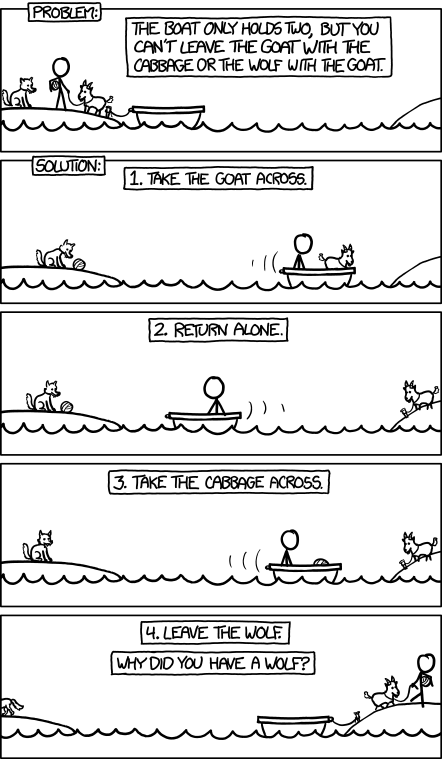
\includegraphics[width=0.6\linewidth]{logic_boat}
  \label{fig:goat}
\end{figure}

Here is the path that they take for this problem. 

\begin{eqnarray*}
 s_0 & = & \msc{On}(\mathrm{Left}, \mathrm{Wolf}) \land \msc{On}(\mathrm{Left}, \mathrm{Goat}) \land \msc{On}(\mathrm{Left}, \mathrm{Cabbage}) \land \msc{On}(\mathrm{Left}, \mathrm{Boat}) \\
a_0 & = &  \msc{Move}(Left, Right, Goat) \\
 s_1 & = & \msc{On}(\mathrm{Left}, \mathrm{Wolf}) \land \msc{On}(\mathrm{Right}, \mathrm{Goat}) \land \msc{On}(\mathrm{Left}, \mathrm{Cabbage}) \land \msc{On}(\mathrm{Right}, \mathrm{Boat}) \\
a_1 & = &  \msc{Move-Empty}(Right, Left) \\
 s_1 & = & \msc{On}(\mathrm{Left}, \mathrm{Wolf}) \land \msc{On}(\mathrm{Right}, \mathrm{Goat}) \land \msc{On}(\mathrm{Left}, \mathrm{Cabbage}) \land \msc{On}(\mathrm{Left}, \mathrm{Boat}) \\
a_2 & = &  \msc{Move}(Left, Right, Cabbage) \\
s_2 & = & \msc{On}(\mathrm{Left}, \mathrm{Wolf}) \land \msc{On}(\mathrm{Right}, \mathrm{Goat}) \land \msc{On}(\mathrm{Right}, \mathrm{Cabbage}) \land \msc{On}(\mathrm{Right}, \mathrm{Boat}) \\
a_2 & = &  \msc{Move}(Right, Left, Cabbage) \\
\end{eqnarray*}

\end{document}